\iffalse
\documentclass[journal,12pt,twocolumn]{IEEEtran}
\usepackage{setspace}
\usepackage{gensymb}
\usepackage{xcolor}
\usepackage{caption}
\singlespacing
\usepackage{siunitx}
\usepackage[cmex10]{amsmath}
\usepackage{mathtools}
\usepackage{hyperref}
\usepackage{amsthm}
\usepackage{mathrsfs}
\usepackage{txfonts}
\usepackage{stfloats}
\usepackage{cite}
\usepackage{cases}
\usepackage{subfig}
\usepackage{longtable}
\usepackage{multirow}
\usepackage{enumitem}
\usepackage{bm}
\usepackage{mathtools}
\usepackage{listings}
\usepackage{tikz}
\usetikzlibrary{shapes,arrows,positioning}
\usepackage{circuitikz}
\renewcommand{\vec}[1]{\boldsymbol{\mathbf{#1}}}
\DeclareMathOperator*{\Res}{Res}
\renewcommand\thesection{\arabic{section}}
\renewcommand\thesubsection{\thesection.\arabic{subsection}}
\renewcommand\thesubsubsection{\thesubsection.\arabic{subsubsection}}

\renewcommand\thesectiondis{\arabic{section}}
\renewcommand\thesubsectiondis{\thesectiondis.\arabic{subsection}}
\renewcommand\thesubsubsectiondis{\thesubsectiondis.\arabic{subsubsection}}
\hyphenation{op-tical net-works semi-conduc-tor}

\lstset{
language=Python,
frame=single, 
breaklines=true,
columns=fullflexible
}
\begin{document}
\theoremstyle{definition}
\newtheorem{theorem}{Theorem}[section]
\newtheorem{problem}{Problem}
\newtheorem{proposition}{Proposition}[section]
\newtheorem{lemma}{Lemma}[section]
\newtheorem{corollary}[theorem]{Corollary}
\newtheorem{example}{Example}[section]
\newtheorem{definition}{Definition}[section]
\newcommand{\BEQA}{\begin{eqnarray}}
        \newcommand{\EEQA}{\end{eqnarray}}
\newcommand{\define}{\stackrel{\triangle}{=}}
\newcommand{\myvec}[1]{\ensuremath{\begin{pmatrix}#1\end{pmatrix}}}
\newcommand{\mydet}[1]{\ensuremath{\begin{vmatrix}#1\end{vmatrix}}}
\bibliographystyle{IEEEtran}
\providecommand{\nCr}[2]{\,^{#1}C_{#2}} % nCr
\providecommand{\nPr}[2]{\,^{#1}P_{#2}} % nPr
\providecommand{\mbf}{\mathbf}
\providecommand{\pr}[1]{\ensuremath{\Pr\left(#1\right)}}
\providecommand{\qfunc}[1]{\ensuremath{Q\left(#1\right)}}
\providecommand{\sbrak}[1]{\ensuremath{{}\left[#1\right]}}
\providecommand{\lsbrak}[1]{\ensuremath{{}\left[#1\right.}}
\providecommand{\rsbrak}[1]{\ensuremath{{}\left.#1\right]}}
\providecommand{\brak}[1]{\ensuremath{\left(#1\right)}}
\providecommand{\lbrak}[1]{\ensuremath{\left(#1\right.}}
\providecommand{\rbrak}[1]{\ensuremath{\left.#1\right)}}
\providecommand{\cbrak}[1]{\ensuremath{\left\{#1\right\}}}
\providecommand{\lcbrak}[1]{\ensuremath{\left\{#1\right.}}
\providecommand{\rcbrak}[1]{\ensuremath{\left.#1\right\}}}
\theoremstyle{remark}
\newtheorem{rem}{Remark}
\newcommand{\sgn}{\mathop{\mathrm{sgn}}}
\newcommand{\rect}{\mathop{\mathrm{rect}}}
\newcommand{\sinc}{\mathop{\mathrm{sinc}}}
\providecommand{\abs}[1]{\left\vert#1\right\vert}
\providecommand{\res}[1]{\Res\displaylimits_{#1}}
\providecommand{\norm}[1]{\lVert#1\rVert}
\providecommand{\mtx}[1]{\mathbf{#1}}
\providecommand{\mean}[1]{E\left[ #1 \right]}
\providecommand{\fourier}{\overset{\mathcal{F}}{ \rightleftharpoons}}
\providecommand{\ztrans}{\overset{\mathcal{Z}}{ \rightleftharpoons}}
\providecommand{\system}[1]{\overset{\mathcal{#1}}{ \longleftrightarrow}}
\newcommand{\solution}{\noindent \textbf{Solution: }}
\providecommand{\dec}[2]{\ensuremath{\overset{#1}{\underset{#2}{\gtrless}}}}
\let\StandardTheFigure\thefigure
\def\putbox#1#2#3{\makebox[0in][l]{\makebox[#1][l]{}\raisebox{\baselineskip}[0in][0in]{\raisebox{#2}[0in][0in]{#3}}}}
\def\rightbox#1{\makebox[0in][r]{#1}}
\def\centbox#1{\makebox[0in]{#1}}
\def\topbox#1{\raisebox{-\baselineskip}[0in][0in]{#1}}
\def\midbox#1{\raisebox{-0.5\baselineskip}[0in][0in]{#1}}

\vspace{3cm}
\title{11.10.3.10}
\author{Lokesh Surana}
\maketitle
\section*{Class 11, Chapter 10, Exercise 3.10}

Q. The line through the points $(h, 3)$ and $(4, 1)$ intersects the line $7{x} - 9{y} - 19 = 0$ at right angle. Find the value of h.

\solution Let the point $\vec{P}$ be the foot of the perpendicular on the line $7{x} - 9{y} - 19 = 0$ from point $\myvec{22/9\\3}$ (Let's say point $\vec{O}$).
The optimization problem can be expressed as

\begin{align}
    \label{eq:grad_dec/optimization}
    \min_{\vec{x}} \norm{\vec{x}-\vec{O}}^2\\
    \text{s.t.} \quad \vec{n}^\top\vec{x} = c
\end{align}

where
\begin{align}
    \vec{n} = \myvec{7 \\ -9},\,c = 19
\end{align}

The line equation can be expressed as
\begin{align}
    \label{eq:grad_dec/line-eq}
    \vec{x} = \vec{A}+\lambda\vec{m}
\end{align}
where
\begin{align}
    \vec{m} = \myvec{9            \\ 7},\,
    \vec{A} = \myvec{\frac{19}{7} \\ 0}
\end{align}

Using the parameric form, Substituting \eqref{eq:grad_dec/line-eq} in \eqref{eq:grad_dec/optimization}, the optimization problem becomes
\begin{align}
    \min_{\lambda} \norm{ \lambda\vec{m} +\brak{\vec{A}-\vec{O}}}^2
\end{align}

\begin{align}
    \begin{split}
        \ \implies \min_{\lambda}f\brak{\lambda} = \lambda^2\norm{\vec{m}}^2 + \\ 2\lambda\brak{\vec{A}-\vec{O}}^\top\vec{m} + \norm{\vec{A}-\vec{O}}^2 \
    \end{split}
\end{align}


yielding
\begin{align}
    f\brak{\lambda} &= 130\lambda^2 -\frac{260}{7}\lambda + \frac{\sqrt{36010}}{63}\\
    f^\prime\brak{\lambda} &= 260\lambda -\frac{260}{7}
\end{align}

\begin{figure}[!htb]
    \centering
    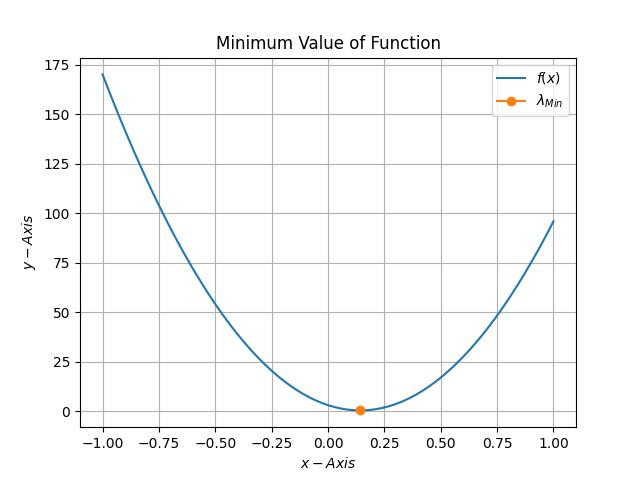
\includegraphics[width=\columnwidth]{figs/plot.jpg}
    \caption{Plot of objective function}
    \label{fig:Plot of objective function}
\end{figure}

Computing $\lambda_{min}$ using Gradient Descent method:
\begin{align}
	\lambda_{n+1} &= \lambda_n - \alpha f^\prime\brak{\lambda_n}\\
    \label{eq:grad_dec/eq1}
	\lambda_{n+1} &= \lambda_n\brak{1-260\alpha} -\frac{260}{7}\alpha
\end{align}

Taking the one-sided $Z$-transform on both sides of \eqref{eq:grad_dec/eq1},
\begin{align}
            \label{eq:grad_dec/Z-trans}
	    z\Lambda\brak{z} &= \brak{1-260\alpha}\Lambda\brak{z} + \frac{260\alpha}{7\brak{1-z^{-1}}} \\
	    \Lambda\brak{z} &= \frac{260\alpha z^{-1}}{7\brak{1-z^{-1}}\brak{1-\brak{1-260\alpha}z^{-1}}} \\
	    &= \frac{1}{7}\brak{ \frac{1}{1-z^{-1}} - \frac{1}{1-\brak{1-260\alpha}z^{-1}}} \\
            \label{eq:grad_dec/lambda-z-trans}
	    &= \frac{1}{7}\sum_{k=0}^{\infty}\brak{1-\brak{1-260\alpha}^k}z^{-k}
\end{align}

From \eqref{eq:grad_dec/lambda-z-trans}, the ROC is
\begin{align}
	\abs{z} &> \max\cbrak{1,\abs{1- 260\alpha}} \\
	\implies -1 & < \abs{1-260\alpha} < 1 \\
        \label{eq:grad_dec/alpha}
        \implies 0 &< \alpha < \frac{1}{130}
\end{align}
Thus, if $\alpha$ satisfies \eqref{eq:grad_dec/alpha}, then from \eqref{eq:grad_dec/lambda-z-trans}, 
\begin{align}
	\label{eq:grad_dec/conv}
        \lim_{n\to\infty}\lambda_n &= \frac{1}{7}
    \end{align}
Choosing
\begin{enumerate}
 \item $\alpha$ = 0.001
 \item precision = 0.0000001
 \item n = 10000000 
 \item $\lambda_0$ = -5 
\end{enumerate}

\begin{align}
	\lambda_{min} &= \frac{1}{7}
\end{align}
Substituting the values of $\vec{A}$, $\vec{m}$ and $\lambda_{min}$ in equation \eqref{eq:grad_dec/line-eq} 
\begin{align}
	\vec{x}_{min} &= \vec{P} = \myvec{\frac{19}{7} \\ 0} +  \frac{1}{7}\myvec{9 \\ 7}  \\
	&= \myvec{4 \\ 1}
\end{align}

This validates that $\vec{P} = \myvec{4\\1}$ is foot of perpendicular from $\vec{O} = \myvec{\frac{22}{9} \\ 3}$ on the line $7{x} - 9{y} - 19 = 0$.
\begin{figure}[!htb]
    \centering
    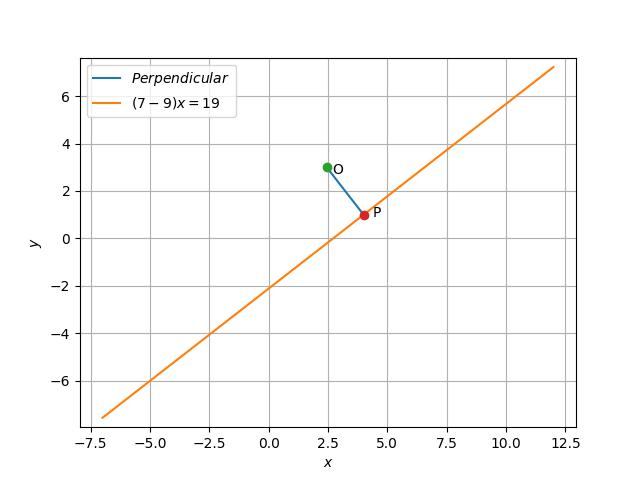
\includegraphics[width=\columnwidth]{figs/lines.jpg}
    \caption{lines}
    \label{fig:lines}
\end{figure}

